\providecommand{\Fun}{\operatorname{Fun}}
\providecommand{\Cat}{\mathcal{C}at}
\providecommand{\QCat}{\mathcal{Q}\mathcal{C}at}
\providecommand{\qcOne}{\mathbf{1}}   %

\section{\trInitial{}\trElement{}与\trTerminal{}\trElement}\label{sec:initial-and-terminal-elements}

沿用定义 1.4.11 定义\trInfinityCategory{}的\trHomotopyCategory{}时所用的策略，
我们用\trTerminal{}∞-\trCategory{} $1$ 来探查一个\trInfinityCategory{} $A$ 的内部。%
\trHomotopyCategory{} $\mathrm{h}A$ 中的一个对象 $a$，定义为∞-\trCategory{}的映射
$a\colon 1\to A$。为了避免「对象」一词的泛滥，并出于对 Lawvere 的（广义）
\trElement{}概念 \cite{bib74} 的敬意，自此以后我们把映射 $a\colon 1\to A$ 称为%
\trInfinityCategory{} $A$ 的\textbf{\trElement}（element）。\footnote{$A$ 的一个%
\trGeneralizedElement{}是一个\trFunctor{} $f\colon X\to A$。由\trYonedaLemma{}，一个%
\trInfinityCategory{}由其诸\trGeneralizedElement{}决定。}这一术语将帮助我们随时把握
所讨论的「范畴层面」：\trElement $a$ 居于\trInfinityCategory{} $A$ 之中，而后者是%
\trInfinityCosmos{} $\mathcal{K}$ 的对象——这些宇宙本身又定义了「无穷维的范畴」，
尽管属于另一种类型。

\begin{definition}[\trInitial{}\trElement／\trTerminal{}\trElement]\label{def:initial-terminal-element}
\trInfinityCategory{} $A$ 中的一个\textbf{\trInitial{}\trElement}（initial element）是唯一%
\trFunctor{} $!\colon A\to 1$ 的一个\trLeftAdjoint{}，如下左图所示；而%
\trInfinityCategory{} $A$ 中的一个\textbf{\trTerminal{}\trElement}（terminal element）是一个%
\trRightAdjoint{}，如下右图所示。
\begin{center}
\begin{tikzpicture}[x=1.4em,y=1.4em]
  \node (L1) at (0,0) {$1$};
  \node (R1) at (3.6,0) {$A$};
  \draw[->] (0.5,0.32) to[bend left=20] node[above]{$i$} (3.1,0.32);
  \node at (1.8,0) {$\dashv$};
  \draw[->] (3.1,-0.32) to[bend left=20] node[below]{$!$} (0.5,-0.32);
  \node (L2) at (7.2,0) {$1$};
  \node (R2) at (10.8,0) {$A$};
  \draw[->] (10.3,0.32) to[bend right=20] node[above]{$!$} (7.7,0.32);
  \node at (9.0,0) {$\dashv$};
  \draw[->] (7.7,-0.32) to[bend right=20] node[below]{$t$} (10.3,-0.32);
\end{tikzpicture}
\end{center}
\end{definition}

让我们拆解\trInitial{}\trElement{}的定义；对偶的评注适用于\trTerminal{}\trElement{}。

\begin{lemma}[最小数据]\label{lem:minimal-data}
要定义一个\trInfinityCategory{} $A$ 中的\trInitial{}\trElement{}，只须指定：
\begin{itemize}
\item 一个\trElement $i\colon 1\to A$；以及
\item 一个\trNaturalTransformation
\begin{center}
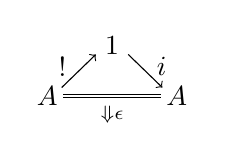
\begin{tikzpicture}[x=1.3em,y=1.3em]
  \node (T) at (1.8,1.4) {$1$};
  \node (L) at (0,0) {$A$};
  \node (R) at (3.6,0) {$A$};
  \draw[->] (0.4,0.24) -- (1.35,1.16);
  \node at (0.42,0.82) {$!$};
  \draw[->] (2.25,1.16) -- (3.2,0.24);
  \node at (3.18,0.82) {$i$};
  \draw[double] (0.45,0) -- (3.15,0);
  \node at (1.8,-0.52) {$\scriptstyle\Downarrow\epsilon$};
\end{tikzpicture}
\end{center}
从常值于 $i$ 的函子到恒同函子，
\end{itemize}
使得其分量 $\epsilon i\colon i\Rightarrow i$——即 $\mathrm{h}A$ 中从 $i$ 到 $i$ 的一个%
箭头——可逆。
\end{lemma}

\begin{proof}
命题 1.4.5——其证明始于该命题陈述之前的一段——表明：\trInfinityCategory{}
$1\in\mathcal{K}$ 在\trHomotopyTwoCategory{} $\mathrm{h}\mathcal{K}$ 中是%
\trTwoTerminalObject{}。这一\trUniversalProperty{}的一维方面蕴含：任何\trElement $i\colon 1\to A$ 都定义了
唯一映射 $!\colon A\to 1$ 的一个\trSection{}；而二维方面则断言：不存在以 $1$ 为
余域的非恒等 2-\trCell{}。特别地，\trAdjunction{} $i\dashv !$ 的\trUnit{}必为恒等，
而\trTriangleEqualities{}之一便自动成立。在此情境下，\cref{def:adjunction}所余的
只是一枚\trCounit{}\trNaturalTransformation{} $\epsilon\colon i!\Rightarrow\mathrm{id}_A$
的数据，连同其分量 $\epsilon i=\mathrm{id}_i$ 这一条件。但事实上，仅从更弱也更
自然的假设——分量 $\epsilon i\colon i\cong i$ 可逆——出发，便可证明这一自然
变换必为恒等。为看清这一点，考虑水平复合
\begin{center}
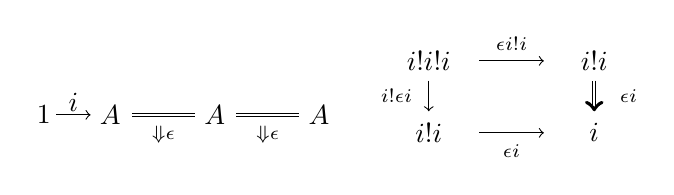
\begin{tikzpicture}[x=1.3em,y=1.3em]
  \node (L1) at (0,0) {$1$};
  \draw[->] (0.35,0) -- (1.3,0);
  \node at (0.82,0.34) {$i$};
  \node (A1) at (1.85,0) {$A$};
  \draw[double] (2.45,0) -- (4.2,0);
  \node at (3.32,-0.55) {$\scriptstyle\Downarrow\epsilon$};
  \node (A2) at (4.75,0) {$A$};
  \draw[double] (5.35,0) -- (7.1,0);
  \node at (6.22,-0.55) {$\scriptstyle\Downarrow\epsilon$};
  \node (A3) at (7.65,0) {$A$};
  \node at (9.15,0) {$\rightsquigarrow$};
  \node (TL) at (10.7,1.5) {$i!i!i$};
  \node (TR) at (15.3,1.5) {$i!i$};
  \node (BL) at (10.7,-0.5) {$i!i$};
  \node (BR) at (15.3,-0.5) {$i$};
  \draw[->] (12.1,1.5) -- (13.9,1.5);
  \node at (13.0,1.98) {$\scriptstyle\epsilon i!i$};
  \draw[->] (10.7,0.95) -- (10.7,0.1);
  \node at (9.8,0.52) {$\scriptstyle i!\epsilon i$};
  \draw[double,->] (15.3,0.95) -- (15.3,0.1);
  \node at (16.25,0.52) {$\scriptstyle\epsilon i$};
  \draw[->] (12.1,-0.5) -- (13.9,-0.5);
  \node at (13.0,-1.0) {$\scriptstyle\epsilon i$};
\end{tikzpicture}
\end{center}
\end{proof}

由\trWhiskering{}的自然性\footnote{「\trWhiskering{}的自然性」（naturality of whiskering）指的是
B.1 节中引理 B.1.3 的观察：2-\trCategory{}中 2-\trCell{}的任何水平复合都可以用
两种不同的方式表达为这些胞腔的若干\trWhiskering{}的竖直复合；在眼下这一情形，它给出了
右上方所展示的 $\mathrm{h}A:=\mathrm{h}\Fun(1,A)$ 中的交换图。
}，我们可以用两种方式把这个复合求值为一个竖直复合。由于 $1$ 是%
\trTwoTerminalObject{}，\trWhiskering{}所得的胞腔 $!\epsilon=\mathrm{id}_!$，于是该复合
关系化归为 $\epsilon i\cdot\epsilon i=\epsilon i$。从而 $\epsilon i$ 是一个
幂等同构，故经消去便是一个恒等。

更简练地说：\trInitial{}\trElement{}定义了\trFunctor{} $!\colon A\twoheadrightarrow 1$ 的一个%
\emph{\trLeftAdjoint{}\trRightInverse}（left adjoint right inverse），而\trTerminal{}\trElement{}定义了一个%
\emph{\trRightAdjoint{}\trRightInverse}（right adjoint right inverse）（见 B.4 节）。

\begin{lemma}[唯一性]\label{lem:uniqueness-of-initial-elements}
\trInfinityCategory{} $A$ 中的任何两个\trInitial{}\trElement{}在 $\mathrm{h}A$ 中同构，而且
$\mathrm{h}A$ 中与某个\trInitial{}\trElement{}同构的任何\trElement{}都是\trInitial{}的。
\end{lemma}
\begin{proof}
由\cref{prop:uniqueness-of-adjoints}，\trFunctor{} $!\colon A\to 1$ 的任何两个%
\trLeftAdjoint{} $i$ 与 $i'$ 自然同构，而任何与 $!\colon A\to 1$ 的一个%
\trLeftAdjoint{}同构的 $a\colon 1\to A$ 本身也是一个\trLeftAdjoint{}。一对\trFunctor{}
$i$ 与 $i'\colon 1\to A$ 之间的\trNaturalTransformation{}同构，恰好给出相应\trElement{}在%
\trHomotopyCategory{} $\mathrm{h}A$ 中的同构 $i\cong i'$ 的数据。
\end{proof}

\begin{remark}\label{rem:representably-initial}
把 2-\trFunctor{} $\Fun(X,-)\colon\mathrm{h}\mathcal{K}\to\mathrm{h}\QCat$ 应用到%
\trInfinityCategory{} $A\in\mathcal{K}$ 的一个\trInitial{}\trElement $i\colon 1\to A$ 上，
便得到一个\trAdjunction
\begin{center}
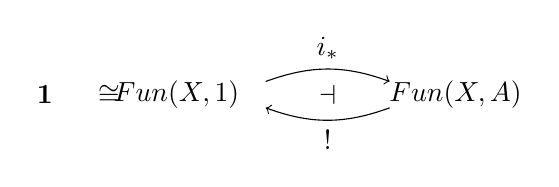
\begin{tikzpicture}[x=1.4em,y=1.4em]
  \node (One) at (0,0) {$\qcOne$};
  \node (F1) at (3.4,0) {$\Fun(X,1)$};
  \node (FA) at (10.6,0) {$\Fun(X,A)$};
  \node at (1.65,0) {$\cong$};
  \draw[->] (5.7,0.34) to[bend left=20] node[above]{$i_{\ast}$} (8.9,0.34);
  \node at (7.3,0) {$\dashv$};
  \draw[->] (8.9,-0.34) to[bend left=20] node[below]{$!$} (5.7,-0.34);
\end{tikzpicture}
\end{center}
经由表达\trTerminal{}∞-\trCategory{} $1$ 之\trUniversalProperty{}的\trIsomorphism{}
$\Fun(X,1)\cong 1$，常值于某个\trInitial{}\trElement{}的\trFunctor
\begin{center}
\begin{tikzpicture}[x=1.4em,y=1.4em]
  \node (X) at (0,0) {$X$};
  \node (One) at (3.4,0) {$1$};
  \node (A) at (6.8,0) {$A$};
  \draw[->] (0.5,0) -- (2.9,0);
  \node at (1.7,0.34) {$!$};
  \draw[->] (3.9,0) -- (6.3,0);
  \node at (5.1,0.34) {$i$};
\end{tikzpicture}
\end{center}
定义了\trFunctorSpace{} $\Fun(X,A)$ 的一个\trInitial{}\trElement{}。这一观察可以概括为：
\trInitial{}\trElement{}在\trInfinityCosmos{}的层面上是\emph{\trRepresentablyInitial}
（representably initial）。

反之，若 $i\colon 1\to A$ 是\trRepresentablyInitial{}，则 $i$ 定义了 $A$ 的一个\trInitial{}\trElement{}。
这一点通过过渡到\trHomotopyTwoCategory{}来看最容易：在其中我们可以证明，一个%
\trInitial{}\trElement $i\colon 1\to A$ 在所有\emph{\trGeneralizedElement}
$f\colon X\to A$ 之中是\trInitial{}的，其确切含义如下。
\end{remark}

\begin{lemma}\label{lem:initial-element-universal-property}
一个\trElement $i\colon 1\to A$ 是\trInitial{}的，当且仅当：对任何 $f\colon X\to A$，
以
\begin{center}
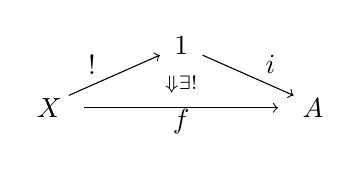
\begin{tikzpicture}[x=1.4em,y=1.4em]
  \node (X) at (0,0) {$X$};
  \node (One) at (3.4,1.6) {$1$};
  \node (A) at (6.8,0) {$A$};
  \draw[->] (0.5,0.32) -- (2.85,1.36);
  \node at (1.1,1.12) {$!$};
  \draw[->] (3.95,1.36) -- (6.3,0.32);
  \node at (5.7,1.12) {$i$};
  \draw[->] (0.9,0) -- (5.9,0);
  \node at (3.4,-0.36) {$f$};
  \node at (3.4,0.6) {$\scriptstyle\Downarrow\exists!$};
\end{tikzpicture}
\end{center}
为边界的 2-\trCell{}存在且唯一。
\end{lemma}

\begin{proof}
若 $i\colon 1\to A$ 是\trInitial{}的，则\cref{def:initial-terminal-element}的%
\trAdjunction{}被 2-\trFunctor{} $\mathrm{h}\Fun(X,-)\colon\mathrm{h}\mathcal{K}\to\Cat$
保持，从而定义了一个\trAdjunction
\begin{center}
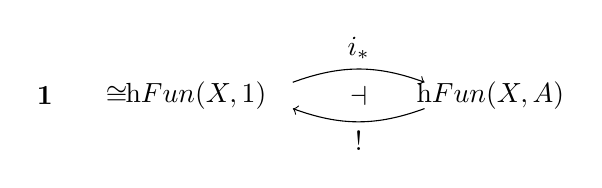
\begin{tikzpicture}[x=1.4em,y=1.4em]
  \node (One) at (0,0) {$\qcOne$};
  \node (F1) at (3.9,0) {$\mathrm{h}\Fun(X,1)$};
  \node (FA) at (11.5,0) {$\mathrm{h}\Fun(X,A)$};
  \node at (1.85,0) {$\cong$};
  \draw[->] (6.4,0.34) to[bend left=20] node[above]{$i_{\ast}$} (9.8,0.34);
  \node at (8.1,0) {$\dashv$};
  \draw[->] (9.8,-0.34) to[bend left=20] node[below]{$!$} (6.4,-0.34);
\end{tikzpicture}
\end{center}
经由\trIsomorphism{} $\mathrm{h}\Fun(X,1)\cong 1$，这个\trAdjunction{}证明了：
\trConstantFunctor{} $i!\colon X\to A$ 在\trCategory{} $\mathrm{h}\Fun(X,A)$ 中是%
\trInitial{}的，从而具有该陈述的\trUniversalProperty{}。

反之，若 $i\colon 1\to A$ 满足该陈述的\trUniversalProperty{}，把它应用于 $A$ 的\trGenericElement{}
（generic element；即恒同映射 $\mathrm{id}_A\colon A\to A$），便产生
\cref{lem:minimal-data}的数据。
\end{proof}

\cref{lem:initial-element-universal-property}说的是：\trInitial{}\trElement{}在%
\trHomotopyTwoCategory{}中是\trRepresentablyInitial{}。把诸\trGeneralizedElement{}特殊化为
通常的\trElement{}，便可见：$A$ 中的\trInitial{}\trElement{}与\trTerminal{}\trElement{}分别定义了其%
\trHomotopyCategory{}中的\trInitial{}\trElement{}与\trTerminal{}\trElement{}：
\begin{rveq}\label{eq:initial-terminal-homotopy-category}
\mbox{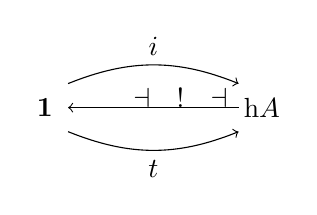
\begin{tikzpicture}[x=1.4em,y=1.4em]
  \node (One) at (0,0) {$\qcOne$};
  \node (hA) at (5.6,0) {$\mathrm{h}A$};
  \draw[->] (0.6,0.62) to[bend left=22] node[above]{$i$} (5.0,0.62);
  \draw[->] (5.0,0) -- (0.6,0);
  \node at (2.5,0.26) {$\dashv$};
  \node at (3.5,0.26) {$!$};
  \node at (4.5,0.26) {$\dashv$};
  \draw[->] (0.6,-0.62) to[bend right=22] node[below]{$t$} (5.0,-0.62);
\end{tikzpicture}}
\end{rveq}

一般而言，「\trHomotopyInitial」（homotopy initial）——即在\trHomotopyCategory{}中%
\trInitial{}——这一性质弱于在\trInfinityCategory{}中\trInitial{}。然而
Nguyen、Raptis 与 Schrade 观察到：\trComplete $(\infty,1)$-\trCategory{}中的一个
同伦\trInitial{}\trElement{}必定定义一个\trInitial{}\trElement \cite[2.2.2]{bib88}。

继续∞-范畴论概念的\trEquivalence{}不变性这一主题：

\begin{lemma}\label{lem:equivalence-invariance-initial-elements}
若 $A$ 有一个\trInitial{}\trElement{}且 $A\simeq A'$，则 $A'$ 有一个\trInitial{}\trElement{}，
并且这些\trElement{}被诸\trEquivalence{}保持至同构。
\end{lemma}
\begin{proof}
由\cref{prop:adjoint-equivalences}，\trEquivalence{} $A\simeq A'$
可以被提升为一个\trAdjointEquivalence{}，而后者立即可与刻画 $A$ 的\trInitial{}\trElement $i$
的那个\trAdjunction{}复合：
\begin{center}
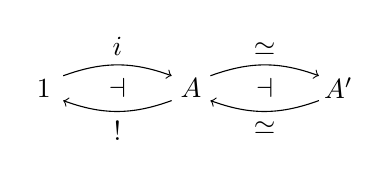
\begin{tikzpicture}[x=1.4em,y=1.4em]
  \node (One) at (0,0) {$1$};
  \node (A) at (3.8,0) {$A$};
  \node (Ap) at (7.6,0) {$A'$};
  \draw[->] (0.5,0.32) to[bend left=20] node[above]{$i$} (3.3,0.32);
  \node at (1.9,0) {$\dashv$};
  \draw[->] (3.3,-0.32) to[bend left=20] node[below]{$!$} (0.5,-0.32);
  \draw[->] (4.3,0.32) to[bend left=20] node[above]{$\simeq$} (7.1,0.32);
  \node at (5.7,0) {$\dashv$};
  \draw[->] (7.1,-0.32) to[bend left=20] node[below]{$\simeq$} (4.3,-0.32);
\end{tikzpicture}
\end{center}
\end{proof}

由\cref{prop:adjunctions-compose}给出的复合\trAdjunction{}证明：$i$ 的像定义了
$A'$ 的一个\trInitial{}\trElement{}，而且由构造，该\trElement{}被\trEquivalence{}
$A\rightsquigarrow A'$ 保持。由\cref{lem:uniqueness-of-initial-elements}所确立的%
\trInitial{}\trElement{}的唯一性，这一论证也表明\trEquivalence{} $A'\rightsquigarrow A$
保持\trInitial{}\trElement{}。

我们现在转向取值于一个\trInfinityCategory{}的\trDiagram{}的\trLimit{}与\trColimit{}的
一般理论。\trInitial{}\trElement{}的理论很好地预演了这一内容：事实上，一个\trInitial{}\trElement
可以被理解为这两个概念各自的实例——\trInitial{}\trElement{}是空图表的\trColimit{}，
同时也是由恒同\trFunctor{}所编码的\trDiagram{}的\trLimit{}，正如我们在\cref{exa:initial-limit-identity}中
所解释的。

\subsection*{练习}

\begin{exercise}\label{ex:representably-initial-element}
用\cref{lem:initial-element-universal-property}证明：如\cref{rem:representably-initial}
所描述的那样，一个可表示地\trInitial{}的\trElement{}必然定义 $A$ 中的一个\trInitial{}\trElement{}。
\end{exercise}

\begin{exercise}\label{ex:preserved-by-adjoints}
证明：\trInitial{}\trElement{}被\trLeftAdjoint{}保持，而\trTerminal{}\trElement{}被%
\trRightAdjoint{}保持。
\end{exercise}
